\documentclass[doc]{apa6}

\usepackage[english]{babel}
\usepackage[utf8x]{inputenc}
\usepackage{amsmath}
\usepackage{graphicx}
\usepackage{apacite}
\usepackage{amsfonts}
\usepackage{url}
%\usepackage[style=apa,sortcites=true,sorting=nyt,backend=biber]{biblatex}
%\DeclareLanguageMapping{american}{american-apa}

  \title{Warm (for Winter): Inferring comparison classes for relative adjectives}
    \author{Michael Henry Tessler\textsuperscript{1}, Michael
Lopez-Brau\textsuperscript{1}, \& Noah D. Goodman\textsuperscript{1}}
    \date{}
  
\shorttitle{ Inferring comparison classes}
\affiliation{
\vspace{0.5cm}
\textsuperscript{1} Department of Psychology, Stanford University}
\keywords{comparison class; pragmatics; Rational Speech Act; Bayesian cognitive model; Bayesian data analysis\newline\indent Word count: X}
\makeatletter
\newcommand\LastLTentrywidth{1em}
\newlength\longtablewidth
\setlength{\longtablewidth}{1in}
\usepackage{tabularx}
\usepackage{multicol}
\usepackage{wrapfig}
\usepackage{gensymb}
\usepackage{tikz}
\usepackage{caption}
\usepackage{booktabs}

\authornote{Complete departmental affiliations for each author
(note the indentation, if you start a new paragraph). Enter author note
here.

Correspondence concerning this article should be addressed to Michael
Henry Tessler, 450 Serra Mall, Bldg. 420, Rm. 316, Stanford, CA 94305.
E-mail:}

\abstract{
The meaning of an utterance can change depending on the context. Yet,
what counts as the relevant context is often only implicit in everyday
conversation. The utterance ``it's warm outside'' could signal many things: It's warm
relative to other days of the year, it's warm for the season, it's warm for the week, etc.. 
\emph{Warm} conveys that the
temperature is high relative to some contextual \emph{comparison class},
but little is known about how a listener decides upon the appropriate
class for comparison. Here, we incorporate a mechanism for inferring the comparison class into a probabilistic model of adjective interpretation, which makes predictions about the relative generality of the comparison class that a listener should prefer.
We test the qualitative predictions of the model in a free production experiment and use a forced-choice version of the task to test the finer-grained, quantitative predictions. 
The resolution of a comparison class requires not only reasoning about what is likely to be the case but also what would be informative to talk about, thus incorporating comparison class inference into the larger study of pragmatic reasoning.
}



\begin{document}
\maketitle

\definecolor{Red}{RGB}{255,0,0}
\definecolor{Green}{RGB}{10,200,100}
\definecolor{Blue}{RGB}{10,100,200}
\definecolor{Orange}{RGB}{255,153,0}

\newcommand{\denote}[1]{\mbox{ $[\![ #1 ]\!]$}}
\newcommand*\diff{\mathop{}\!\mathrm{d}}
\newcommand{\red}[1]{\textcolor{Red}{#1}}  
\newcommand{\ndg}[1]{\textcolor{Green}{[ndg: #1]}}  
\newcommand{\mht}[1]{\textcolor{Blue}{[mht: #1]}}  
\newcommand{\mlb}[1]{\textcolor{Orange}{[mlb: #1]}}

\section{Introduction}

A 75 \degree F (24 \degree C) day is warm. A 60 \degree F (16 \degree C)
day is not, unless it's January; it could be warm for January.
\emph{Warm} is relative, and its felicity depends upon what the speaker
uses as a basis of comparison---the \emph{comparison class} (e.g., other
days of the year or other days in January). Comparison classes are
necessary for understanding adjectives and, in fact, any part of
language whose meaning must be pragmatically reconstructed from context,
including vague quantifiers \cite<e.g., ``He ate a lot of burgers.'';>{Scholler2017} and generic language \cite<e.g., ``Dogs are friendly''>{Tessler2019psychrev}. Deciding on the relevant
comparison class is a case study in the larger question of inferring the
appropriate aspects of context for interpreting an utterance. Comparison
classes, as with relevant aspects of context more generally, often go
unsaid (e.g., in ``It's warm outside'').

The existence of comparison classes for understanding vague language is
uncontroversial \cite{Bale2011, Solt2009} \red{more standard citations for this?}. 
Adult judgments of the felicity for adjectives like ``dark'' or ``tall'' depend
upon fine-grained details of the statistics of the comparison class:
When objects in the comparison class are all rather short, what counts
as ``tall'' might not be very tall \cite{Qing2014b, Schmidt2009, Solt2012}.
Four-year-olds use their knowledge of kinds to differentiate between
what goes into the comparison class and what does not: What counts as a
``tall pimwit'' depends on the distribution of heights of
\emph{pimwits} and not the heights of other creatures like \emph{daxes}
\cite{Barner2008}. Even children as young as 2-and-a-half
understand that ``big'' is relative ({\textbf{???}}) and that the
comparison class can change \cite<e.g., a ``small mitten'' can be big for the
current physical context;>{Ebeling1988, Ebeling1994}.

How do listeners decide on the appropriate comparison class? Any
particular referent of discourse can be conceptualized or categorized in
multiple ways, giving rise to multiple possible comparison classes. A day in
January is also a day of the year; if a listener hear ``It's
warm'', it could be \emph{warm for the week}, \emph{warm for winter}, or
\emph{warm for the year}.\footnote{It could also be \emph{warm for
  Boston}, \emph{warm for the northeast USA}, \emph{warm for a place
  with currently six inches of snow on the ground}, among many more
  possibilities. } In this paper, we investigate the first aspect of
this problem, deciding among multiple plausible, conceptual comparison
classes. Theoretical work in semantics has focused on how information
from the comparison class gets integrated with a compositional semantics
and what representations might be preferred \cite{Bale2011, Solt2009}.
The question of how listeners reconstruct a comparison class in
undersupported contexts (e.g., just hearing ``It's warm outside'')
has been addressed neither formally nor empirically.

We propose that listeners combine probabilistic, category knowledge with
pragmatic reasoning to infer the comparison class implicitly used by the
speaker. This proposal leads to the following prediction: When it is
winter, saying ``it's warm'' signals that it is \emph{warm for
winter}, while saying ``it's cold'' signals \emph{cold for the
year}. The opposite relationship should hold in summer, where
``it's cold'' should signal it's cold \emph{for summer} more so
than ``it's warm''. This prediction is a result of the \emph{a
priori} probability of different temperatures in different seasons: In
winter, temperatures are relatively low, and thus it is unlikely to
actually be \emph{warm for the year}. In addition, regardless of the
season and the adjective (e.g., ``warm'' or ``cold''),
listeners prefer comparison classes that are relatively specific (e.g.,
relative to \emph{the current season} as opposed to \emph{the whole
year}); more specific comparison classes have lower variance, and a
vague adjectives like \emph{warm} carries more information when it is
interpreted with respect to a lower variance comparison class. These
predictions fall out of a Rational Speech Act (RSA) model for gradable
adjectives \cite{Lassiter2013, Lassiter2017}, extended to flexibly
reason about the implicit comparison class. We test these predictions in
two experiments by eliciting the comparison class using a forced-choice
paraphrase dependent measure (Expt. 1) and a free-production dependent
measure using an expanded stimulus set (Expt. 2).

\textcolor{Blue}{[mht: move to end of first expt]}

The model's quantitative predictions can be generated by explicitly
specifying the interlocutors' relevant prior knowledge (e.g., beliefs
about temperatures). The current methodological standard is to measure
beliefs by having participants estimate quantities or give likelihood
judgments \cite{Franke2016}. We pursue a different methodology. The
RSA model captures a productive fragment of natural language; thus, it
makes predictions about a related natural language task (Expt. 2).
Critically, we can use the model to predict natural language judgments
that require the \emph{same prior knowledge} as in Expt. 1 and use
Bayesian data analysis to jointly infer the shared priors. This approach
harnesses the productivity of language into experiment design and allows
us to reconstruct priors without having participants engage in
challenging numerical estimation tasks.

\section{Computational Model}

Gradable adjectives like \emph{warm} and \emph{cold} are vague
descriptions of an underlying quantitative scale (e.g., temperature).
The vagueness and context-sensitivity of these adjectival utterances can
be modeled using threshold semantics (\([\![u]\!] = x > \theta\), for
utterance \(u\), scalar degree \(x\), and threshold \(\theta\)), where
the threshold is probabilistically set with respect to a comparison
class \(c\) via pragmatic reasoning (Lassiter \& Goodman, 2013; see also
Qing \& Franke, 2014a):

\begin{align}
L_{1}(x, \theta \mid u) &\propto S_{1}(u \mid x, \theta) \cdot P_{c}(x) \cdot P(\theta) \label{eq:L1} \\
S_{1}(u \mid x, \theta) &\propto \exp{(\alpha_1 \cdot \ln {L_{0}(x \mid u, \theta)} - \text{cost}(u))} \label{eq:S1}\\
L_{0}(x \mid u, \theta) &\propto {\delta_{[\![u]\!](x, \theta)} \cdot P_{c}(x)} \label{eq:L0}
\end{align}

Eqs. \ref{eq:L1} - \ref{eq:L0} are a Rational Speech Act (RSA) model, a
recursive Bayesian model where speaker \(S\) and listener \(L\)
coordinate on an intended meaning of an utterance \(u\) (for a review,
see Goodman \& Frank, 2016). In this model, a pragmatic listener \(L_1\)
tries to resolve the state of the world \(x\) (e.g., the temperature)
from the utterance she heard \(u\) (e.g., ``it's warm''). He
imagines the utterance came from an approximately rational Bayesian
speaker \(S_1\) trying to inform a naive listener \(L_0\), who in turn
updates his prior beliefs \(P_c(x)\) via an utterance's literal meaning
\([\![u]\!](x, \theta)\).\footnote{We use the male pronoun ``he''
  to refer to listeners and the female pronoun ``she'' to refer to
  speakers.} Formally, the literal meaning is represented by the
Kronecker delta function \(\delta_{\mbox{ $[\![ u ]\!]$}(x, \theta)}\)
that returns probabilities proportional to \(1\) when the utterance is
true (i.e., when \(x > \theta\)) and \(0\) otherwise.

The key innovation used for modeling context-sensitive literal meanings
(as in the case of gradable adjectives) is to have uncertainty over the
semantic variable---the threshold \(\theta\) (Eq. \ref{eq:L1}). In
Lassiter and Goodman (2013)'s model, \(\theta\) comes from an uniform
prior distribution over possible thresholds and is resolved by the
listener reasoning about the different thresholds a speaker might be
using \(S_{1}(u \mid x, \theta)\) as well as the probabilities of
different states of the world \(P_{c}(x)\) (e.g., different
temperatures). Assuming the adjective adds some cost to the speaker's
utterance (Eq. \ref{eq:S1}), the meaning of a gradable adjectives (e.g.,
``warm'') is resolved by the pragmatic listener to mean something
like ``significantly greater temperature than one might expect''
(Lassiter \& Goodman, 2015). Critically, what ``one might
expect''---the prior distribution over temperatures \(P_{c}(x)\)---is
always with respect to some comparison class \(c\) (Eqs. \ref{eq:L1} \&
\ref{eq:L0}). Where does this comparison class come from?

We hypothesize that listeners maintain uncertainty about multiple
possible comparison classes, but can reduce their uncertainty by
combining world knowledge with pragmatic reasoning. More specifically,
listeners use their world knowledge of what worlds are plausible under
different comparison classes \(P(x \mid c)\) (e.g., the likelihood of
different temperatures within different seasons), what implicit
comparison classes are likely to be talked about \emph{a priori}
\(P(c_i)\) (\(i\) for implicit), and how a rational speaker would behave
in a given world assuming a particular comparison class
\(S_{1}(u \mid x, c_i, \theta)\) (Eq. \ref{eq:L1a}). To explore this
model, we consider an idealized case where the comparison class can be
either a relatively specific (subordinate, \(c_{sub}\)) or relatively
general (superordinate, \(c_{super}\)) categorization (e.g., warm
relative to \emph{days in winter} or relative to \emph{days of the
year}): \(c_i \in \{c_{sub}, c_{super}\}\). As in previous models, we
assume the listener is aware that the referent is a member of the
subordinate class (and by extension, the superordinate as well). We
additionally assume the pragmatic listener uses the most subordinate
class information to inform the likely values of the degree (e.g., the
listener's prior over temperatures is given by the distribution of
temperatures for a specific class such as \emph{winter}
\(P(x \mid c = c_{sub})\)). With these assumptions, the model becomes:

\begin{align}
L_{1}(x, c_{i}, \theta \mid u) &\propto S_{1}(u \mid x, c, \theta) \cdot P(x \mid c =  c_{sub}) \cdot P(c_{i}) \cdot P(\theta) \label{eq:L1a}\\
S_{1}(u \mid x, c_i, \theta) &\propto \exp{(\alpha_1 \cdot \ln {L_{0}(x \mid u, c_i, \theta)}- \text{cost}(u)) } \label{eq:S1a}\\
L_{0}(x \mid u, c_i, \theta) &\propto {\delta_{[\![u]\!](x, \theta)} \cdot P(x \mid \text{parseClass}(u, c_i))} \label{eq:L0a}
\end{align}

We are interested in the behavior of the pragmatic listener model with
he hears an utterance without an explicit comparison class \(u_{i}\)
(e.g., ``It's warm''). The listener reasons about alternative
utterances the speaker could have said in order to draw pragmatic
inferences. In this model, we assume the speaker has the option of
conveying the adjective with an explicit comparison class \(u_{sub}\)
and \(u_{super}\) (e.g., ``It's warm relative to other days in
winter'' and ``It's warm relative to other days of the year'').
The literal meanings of these alternatives are the same as the
underspecified utterance (i.e., a threshold function:
\([\![u_{warm}]\!] = x > \theta\)), but have the additional feature of
overriding the implicit comparison class \(c_i\)and forcing the literal
listener into a particular comparison class encoded in the utterance via
the function \(\text{parseClass}\). That is:

\begin{eqnarray}
\text{parseClass}(u, c_i) & = &
\begin{cases}
c_{i} & \text{if } u = u_{i}\\
c_{sub} & \text{if } u = u_{sub}\\
c_{super} & \text{if } u = u_{super}\\
\end{cases}
\end{eqnarray}

Thus, the speaker conditioning on a particular value for \(c_{i}\) only
has implications for the literal listener if the speaker chooses to
produce the implicit utterance (e.g., ``It's warm''). Should the
speaker instead choose an utterance that explicitly articulates the
comparison class (e.g., ``It's warm for winter''), the literal
listener will use the explicit class to set his prior expectations
\(P(x \mid c)\) via the \(\text{parseClass}\) operator.

\begin{figure}
\centering
\includegraphics{figs/speakerSimulations-1.pdf}
\caption{\label{fig:speakerSimulations}Speaker model behavior assuming
different comparison classes. The underspecified utterance
(``warm'') takes on the same meaning of the explicit utterance
whose comparison class is the same as the implicit class (e.g., if the
speaker is using the (for winter) comparison class, ``warm'' means
the same thing as ``warm for winter''). When the speaker is
assuming winter is the comparison class, when the temperature is low, she
will say ``warm'' or ``warm for winter'', but if the
temperature is relatively high, she will only say ``warm for the
year''. When the speaker is assuming the year is the comparison class,
and the temperature is relatively low, she will say ``warm for
winter''. The listener believes temperature is relatively low (believes
it is winter), and inverts this model of speaker to conclude that the
implicit comparison class was winter. The specific class in this example
(winter) is a Normal distribution centered at -1, and the general class
(the year) is a Normal centered at 0.}
\end{figure}

\subsubsection{Qualitative model
predictions}

To understand the model behavior, consider the speaker model \(S_1\)
under different assumptions (by the listener) about the implicit
comparison class: \(S_{1}(u \mid x, \theta, c_i = c_{sub})\) and
\(S_{1}(u \mid x, \theta, c_i = c_{super})\). For illustrative purposes,
we will assume the speaker model can produce utterances with adjectives
of both the positive and negative forms (e.g., \emph{warm} and
\emph{cold}).\footnote{Following standard treatment of antonyms, the
  semantics of ``cold} are a threshold function on a distinct
  threshold variable: \([\![u_{cold}]\!] = x < \theta_{cold}\)), which
  is also inferred via the pragmatic listener (i.e., the listener infers
  a threshold for both ``warm'' and ``cold''). The pragmatic
  inferences about the comparison class that are the focus of this paper
  are invariant to whether or not the antonym is included in the
  alternative set. The comparison class inferences are also invariant to
  whether or not the antonym gets assigned its own unique threshold
  (\(\theta_{cold}\)), as well as whether or not the utterances with
  explicit comparison classes get assigned their own thresholds (e.g., a
  \(\theta_{warm}^{sub}\) and \(\theta_{warm}^{super}\)). Figure
\ref{fig:speakerSimulations} shows the speaker production probabilities
of the six possible utterances for each value along the degree scale
(e.g., each temperature) for the two different implicit classes. The
utterance which does not reference a class (e.g., ``It's warm'')
inherits the same meaning as the utterance with the explicit class that
matches the assumed implicit class (i.e., if \(c_{i} = c_{sub}\), then
\(u_i\) has the same meaning as \(u_{sub}\)). Therefore, reasoning about
the likely comparison class reduces to reasoning about which explicit
utterance the speaker would have been more likely to say. If the
subordinate class in question is ``winter'', the speaker will want
to produce utterances with the subordinate class when the temperatures
are typical winter temperatures (e.g., roughly \(x < -0.5\)). Since the
implicit utterance given a particular implicit class takes on the same
meaning as an explicit utterance, the speaker will be likely to produce
implicit utterances when the implicit class is the subordinate. Thus,
there is an overall preference for speakers to have meant something
about the subordinate class.

A listener who hears either ``it's warm outside'' or ``it's
cold outside'' (during winter), however, will draw different inferences
about the comparison class. Since the listener knows it's winter, the
temperature is likely to be relatively low; ``warm'' is much more
likely to be true if it's ``warm for winter'' than if it's
actually ``warm for the year''. The utterance ``it's cold
outside'' is predicted to be far more ambiguous, because a cold day in
winter is also very likely to be cold for the year. In general, hearing
a positive-form adjective (``warm'') when the mean of the
subordinate class is low (e.g., temperatures in winter) will signal the
subordinate class (warm \emph{for winter}) more so than hearing the
negative-form (``it's cold''; Prediction 1). All else being equal,
however, listeners will prefer subordinate comparison classes
(Prediction 2) because they represent the most specific category of
shared knowledge between speaker and listener; more specific classes
have lower variance (by definition) and vague utterances about lower
variance classes carry relatively more information than higher variance
classes. Figure \ref{fig:modelSchematics} (right) shows that subordinate
class interpretations are above baseline regardless of the adjective
polarity (positive or negative) or the mean of the subordinate prior
(low, medium, high). We test these two predictions in a pre-registered
experiment.

\begin{table*}[ht]
\centering
\begin{tabularx}{\textwidth}{lll}
  \hline
Scale (adjectives) & Subordinate classes & Superordinate \\ 
  \hline
Height (tall, short) & (professional) gymnast, soccer player, basketball player & people \\ 
  Price (expensive, cheap) & bottle opener, toaster, dishwasher & kitchen appliances \\ 
  Temperature (warm, cold) & winter, fall, summer (day in Maryland) & days in the year \\ 
  Time (long, short) & video of a cute animal, music video, movie & things you watch online \\ 
  Weight (heavy, light) & grape, apple, watermelon & produce \\ 
   \hline
\end{tabularx}
\caption{Items used in Experiments 1 and 2. Subordinate categories were designed to fall near the low end, high end, and somewhere in the middle of the degree scale} 
\label{tab:1}
\end{table*}

\begin{figure*}[htb]

{\centering 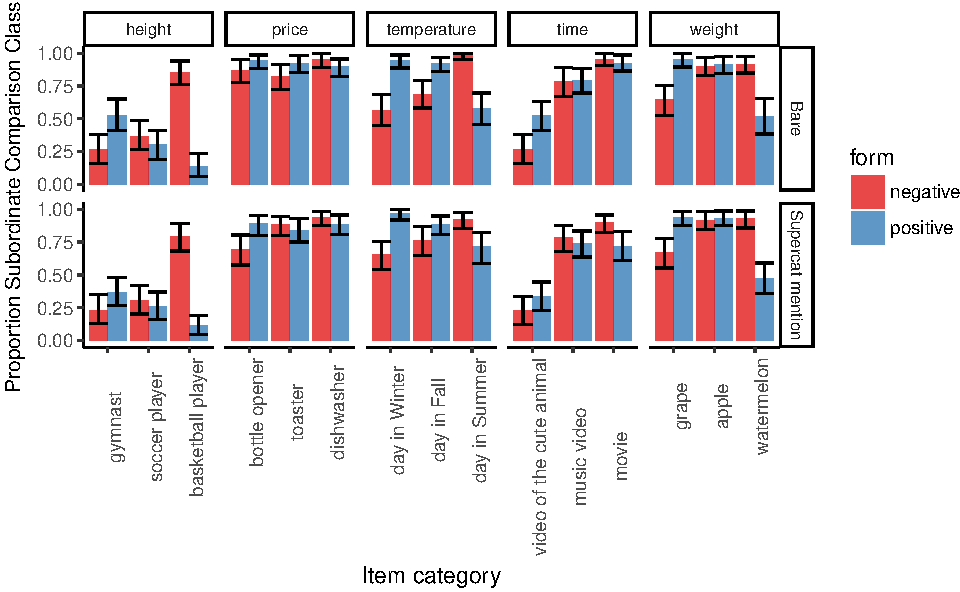
\includegraphics[width=1\textwidth]{figs/expt1results-1} 

}

\caption{Empirical comparison class judgments in terms of proportion in favor of subordinate comparison class.  Error bars correspond to 95\% Bayesian credible intervals.}\label{fig:expt1results}
\end{figure*}

\begin{figure*}[htb]

{\centering \includegraphics[width=1\textwidth]{figs/modelParameters-1} 

}

\caption{Reconstructed degree priors (top) and empirically derived comparison class priors (botton). Top: Inferred prior distributions of world knowledge used to model Experiment 1 and 2 data. Bottom: Inferred prior probability of the subordinate comparison classes based on Google WebGram frequencies. Error bars correspond to 95\% Bayesian credible intervals, derived from the posterior on the $\beta$ scale parameter.}\label{fig:modelParameters}
\end{figure*}

\section{Behavioral experiment}

We gathered human judgments of comparison classes in ambiguous contexts
in a pre-registered test of our two predictions described in
\textbf{Qualitative Model Predictions} (\url{osf.io/k8mnz/}).



\subsubsection{Participants}

We recruited 264 participants, 2 of whom were excluded for failing an
attention check. Participants were recruited from Amazon's Mechanical
Turk and were restricted to those with U.S. IP addresses with at least a
95\% work approval rating. Each experiment took about 5 minutes and
participants were compensated \$0.50 for their work.



\subsubsection{Materials}

We used positive- and negative-form gradable adjectives describing five
scales (Table \ref{tab:1}). Each scale was paired with a superordinate
category, and for each superordinate category, we used three subordinate
categories that aimed to be situated near the high-end, low-end, and
intermediate part of the degree scale (as in Figure
\ref{fig:modelSchematics} left). This resulted in 30 unique items (\{3
subordinate categories\} x \{5 scales\} x \{2 adjective forms\}). Each
participant saw 15 trials: one for each subordinate category paired with
either the positive or negative form of its corresponding adjective.
Participants never judged the same subordinate category for both
adjective forms (e.g., cold and warm winter days) and back-to-back
trials involved different scales to avoid fatigue.


\subsubsection{Procedure}

On each trial, participants were given a context sentence to introduce
the subordinate category (e.g., ``Tanya lives in Maryland and
steps outside in winter''). This was followed by an adjective sentence,
which predicated either a positive- or negative-form gradable adjective
over the item (e.g., ``Tanya says to her friend, ``It's
warm.''). Participants were asked ``What do you think Tanya
meant?'' and given a two-alternative forced-choice to rephrase the
adjective sentence with either an explicit subordinate or superordinate
comparison class:

\begin{quote}
\{She / He / It\} is \textsc{adjective} (e.g., warm) relative to other
\textsc{subordinates} (e.g., \emph{days in winter}) or
\textsc{superordinates} (e.g., \emph{days of the year})
\end{quote}

In addition to all of the above design parameters, half of our
participants completed trials where an additional sentence introduced
the superordinate category at the beginning (e.g., \emph{Tanya lives in
Maryland and checks the weather every day.}), with the intention of
making the superordinate paraphrase more salient.

\begin{figure*}[htb]

{\centering \includegraphics{figs/posteriorPredictiveScatters-1} 

}

\caption{Human endorsement of subordinate comparison class paraphrases (middle; Expt. 1) and adjective sentences (left; Expt. 2) as a function of listener model $L_1$ and speaker model $S_2$ predictions, respectively. The right facet displays a subset of the paraphrase data (Expt. 1) to reveal good quantitative fit even in a small dynamic range. Error bars correspond to 95\% Bayesian credible intervals.}\label{fig:posteriorPredictiveScatters}
\end{figure*}



\subsubsection{Results}

We observed no systematic differences between participants' responses
when the superordinate category was previously mentioned in the context
and those when it was not; thus, we collapse across these two conditions
for all analyses. Figure \ref{fig:expt1results} shows the proportion of
participants choosing the \emph{subordinate} paraphrase for each item,
revealing considerable variability both \emph{within}- and
\emph{across}- scales. The predicted effects are visually apparent
within each scale (compare with Figure \ref{fig:modelSchematics} right).

Our qualitative predictions are confirmed using a generalized linear
mixed effects model with main effects of adjective form (positive
vs.~negative) and the \emph{a priori} judgment by the first author of
whether the sub-category was expected to be low or high on the degree
scale, and of critical theoretical interest, the interaction between
these two variables. In addition, we included by-participant random
effects of intercept and by-subordinate category random effects of
intercept and interaction between form and strength\footnote{This was
  the maximal mixed-effects structure that converged.}. Confirming our
two qualitative model predictions, there was an interaction between form
and strength (\(\beta = -3.82\); \(SE = 0.57;\) \(z = -6.73\)) and there
was an overall preference for subordinate category paraphrases
(\(\beta = 1.23\); \(SE = 0.45;\) \(z = 2.70\)). The main effects of
form and strength were not significant.

We then test the simple effects. For items low on the degree scale
(e.g., temperatures in winter), positive form adjectives were
significantly more likely to imply subordinate comparison classes
(\(\beta = 1.41\); \(SE = 0.15;\) \(z = 9.43\)), while the opposite is
true for items high on the scale (e.g., summer days; \(\beta = -2.50\);
\(SE = 0.19;\) \(z = -13.15\)). Participants reason pragmatically to
resolve the comparison class, combining world knowledge with
informativity as predicted by our model.


\section{Quantitative modeling}

The behavioral experiment bore out our two qualitative predictions
derived from the comparison class inference model. The model is a
quantitative model, however, and can make quantitative predictions
concerning the strength of comparison class inferences. Indeed, we
observe substantial variability in the predicted inferences both within-
and across- scales. Here we test whether the observed variability in
inferences can be accounted for by the constructs posited in our model.
We describe the two relevant constructs---the comparison class prior
\(P(c)\) and the degree priors \(P(x \mid c)\)---before outlining our
Bayesian data analytic strategy.

\subsubsection{Comparison class prior}

\(P(c)\) reflects listeners' expectations of what classes are likely to
be discussed. As a proxy for comparison class usage frequency, we use
empirical frequency \(\hat{f}\) estimated from the Google WebGram
corpus\footnote{Corpus accessed via
\url{https://corpora.linguistik.uni-erlangen.de/cgi-bin/demos/Web1T5/Web1T5_freq.perl}. Due to potential polysemy and idiosyncracies of our experimental
  materials (Table 1), we made the following substitutions when querying
  the database for empirical frequency: produce $\rightarrow$
  ``fruits and vegetables''; things you watch online
  $\rightarrow$ ``online videos''; days in \{season\}
  $\rightarrow$ ``\{season\} days''; dishwashers $\rightarrow$
  ``dishwashing machines''; videos of cute animals $\rightarrow$
  ``animal videos''.}, and scale it by a free parameter $\beta$
such that $P(c) \propto \exp{(\beta \cdot \log \hat{f})}$.


\subsubsection{Degree priors (World
knowledge)}

Only the relative values for \(P(x \mid c_{sub})\) and
\(P(x \mid c_{super})\) affect model predictions. Hence we fix each
superordinate distribution to be a standard normal distribution
\(P(x \mid c_{super}) = \mathcal{N}(0, 1)\) and the subordinate priors
to also be Gaussian distributions
\(P(x \mid c_{sub}) = \mathcal{N}(\mu_{sub}, \sigma_{sub})\); the
subordinate priors thus have standardized units.

\subsubsection{Overview of data analytic
approach}

Specifying the relevant prior knowledge yields two free parameters per
subordinate class. We put priors over these parameters and infer their
likely values using Bayesian data analysis. The data from the comparison
class inference experiment would be insufficient, however, to reliably
estimate all of the parameters of this data analytic model. To alleviate
this, we use the same RSA model to predict additional data about related
language used in the same domains. Specifically, we gather judgments
about adjectives when the comparison class is explicit (\(n = 100\)):
whether or not an adjective would apply to a subordinate member
explicitly relative to the superordinate category (e.g., Is a day in
winter warm relative to other days of the year?).\footnote{The judgments
  in this experiment were consistent with the \emph{a priori} ordering
  of the subordinate categories on the degree scale (e.g., a day in
  winter is likely to be cold for the year).}

To model this adjective endorsement data, we remove comparison class
uncertainty by setting \(P(c_{super}) = 1\), since the sentence being
endorsed include an explicit comparison to the superordinate class. We
model sentence endorsement using a pragmatic speaker (following Qing \&
%Franke, 2014a; Tessler \& Goodman, 2016a, 2016b): \vspace{-0.5cm}
\begin{equation}
S_{2}(u \mid c_{sub}) \propto \exp{(\alpha_2 \cdot {\mathbb E}_{x\sim P_{c_{sub}}} \ln{L_1(x \mid u)})} \label{eq:S2}
\end{equation} 



\noindent Note that $L_1(x \mid u)$ is defined from Eq.
\ref{eq:L1a} by marginalization.

Eqs. \ref{eq:L1a} and \ref{eq:S2} define models for the comparison class
inference task and adjective endorsement task, respectively, and depend
on the same background knowledge \(P(x\mid c)\). We can thus use data
from both experiments to jointly reconstruct the shared prior knowledge
and generate predictions for the two data sets.


\section{Full model analysis and
results}

The RSA listener (Eq. \ref{eq:L1a}) and speaker (Eq. \ref{eq:S2}) models
make quantitative predictions about comparison class interpretation and
adjective endorsement, respectively. We construct a single data-analytic
model with each of these RSA components as sub-models in order to make
quantitative predictions about the data from both of our experiments.

The listener and speaker sub-models share their prior world knowledge
\(P(x \mid c)\) (e.g., temperatures in winter), described in the
\textbf{Degree Priors} section. We put the same priors over the
parameters of each subordinate distribution:
\(\mu \sim \text{Uniform}(-3, 3)\),
\(\sigma \sim \text{Uniform}(0, 5)\), since they have standardized
units. The comparison class prior \(P(c)\) in Eq. \ref{eq:L1a} scales
the empirical frequency \(\hat{f}\) by a free parameter, which we give
the following prior: \(\beta \sim \text{Uniform}(0, 3)\).

The full model has three additional parameters not of direct theoretical
interest: the speaker optimality parameters \(\alpha^\text{expt}_{i}\),
which can vary across the two tasks. The pragmatic listener \(L_1\)
model (Eq. \ref{eq:L1a}) has one speaker optimality:
\(\alpha^\text{1}_{1}\). The pragmatic speaker \(S_2\) model (Eq.
\ref{eq:S2}) has two speaker optimality parameters:
\(\{\alpha^\text{2}_{1}, \alpha^\text{2}_{2}\}\). We use priors
consistent with the previous literature:
\(\alpha_1 \sim \text{Uniform}(0, 20)\),
\(\alpha_2 \sim \text{Uniform}(0, 5)\)

We implemented the RSA and Bayesian data analysis models in the
probabilistic programming language WebPPL (Goodman \& Stuhlmuller,
2014). To learn about the credible values of the parameters, we
collected 2 chains of 50k iterations (after 25k burn-in) using an
incrementalized version of MCMC (Ritchie, Stuhlmuller, \& Goodman,
2016).

\subsubsection{Results}

The full model's posterior over the RSA and data-analytic parameters
were consistent with prior literature and intuition. The maximum
a-posteriori (MAP) estimate and 95\% highest probability density (HPD)
intervals for model parameters specific to the \(L_1\) model used for
comparison class inference were \(\alpha^{1}_{1} = 1.60 [1.10, 2.50]\),
\(\beta = 0.13 [0.11, 0.19]\). Model parameters specific to the \(S_2\)
model used for adjective endorsement:
\(\alpha^{2}_{1} = 3.50 [0.60, 13.20]\),
\(\alpha^{2}_{2} = 3.20 [2.60, 3.80]\). The inferred distributions
corresponding to subordinate class priors were consistent with the
\emph{a priori} ordering of these subordinate classes (low, medium,
high) used in these tasks (Figure \ref{fig:modelParameters} top).

Finally, the full model's posterior predictive distribution does an
excellent job at capturing the quantitative variability in comparison
class inferences: \(r^2(30) = 0.96\), and adjective endorsements:
\(r^2(30) = 0.98\) (Figure \ref{fig:posteriorPredictiveScatters}).
Because of the overall preference for the subordinate comparison class,
many of the data points are distributed above 0.5. Even for these
fine-grained differences, the model does a good job at explaining the
quantitative variability in participants' data (Figure
\ref{fig:posteriorPredictiveScatters} right). Thus, the variability in
comparison class inferences we observe in our behavioral data can be
accounted for the constructs posited in our model (namely, the
comparison class prior and degree priors).

\section{Discussion}

Investigations of how human listeners understand vague adjectives have
shed light on the precise mechanisms by which people interpret
context-sensitive language, but have had little to say about how
listeners decide upon what counts as the appropriate context. In this
paper, we take the first step towards investigating the flexibility in
the class against which an entity can be implicitly compared, a very
basic form of context. We introduced a minimal extension to an adjective
interpretation Rational Speech Act model to allow it to flexibly reason
about the comparison class. This model made the novel prediction that
listeners should try to accomodate a vague utterance by choosing the
comparison class most likely to make the utterance true while
prioritizing more specific (lower variance) classes because they are
more informative. It also made quantitative predictions about how
background knowledge about the degree scale and what classes are likely
to be talked about \emph{a priori} should inform this inference in a
graded fashion. Both qualitative predictions of the model were borne out
in our behavioral experiment, and the quantitative predictions were
confirmed using a novel data analytic technique.

Resolving underspecification by means of a comparison is not unique to
\emph{gradable adjectives} like ``big'' or ``tall'', but is
a general problem for language understanding. ``John ate \emph{a
lot} of hot dogs'' probably means four or five hot dogs, whereas
``John ate \emph{a lot} of potato chips'' could imply a quantity
over a hundred (Schöller \& Franke, 2017); ``Robins lay eggs''
means roughly that \emph{female robins} lay eggs, whereas
``Robins fly'' entails something stronger, most or all robins fly
({\textbf{???}}; {\textbf{???}}). Even noun concepts (e.g.,
``furniture'') are graded (Rosch \& Mervis, 1975) and can be made
more precise in context. Investigating how listeners interpret words
like ``big'' is thus a case study of a crucial, general problem in
language understanding: Understanding context-sensitive language.

We investigated the question of how a listener decides among multiple
possible conceptually-based comparison classes (e.g., tall for a
basketball player vs.~tall for a person). It is notable that our model
was able to account for inferences about items that did not fall into
strict hierachies (e.g., \emph{movies} is not subordinate to
\emph{things you watch online}) as well as items that did (e.g.,
basketball players and people). This result suggests that our modeling
framework can easily extend into cross-cutting comparison classes (e.g.,
\emph{men}, \emph{people of a certain age}, \emph{basketball players}).

\subsection{The phenomenon of comparison class
inference}

To our knowledge, we present the first behavioral data of how reference
classes for adjective interpretation can adjust based on world
knowledge. Previous experimental work on adjective understanding in
young children has looked at what counts as being in the comparison
class (e.g., the comparison class for a ``tall pimwit'' is \emph{other
pimwits} and not \emph{other creatures in general}; Barner \& Snedeker,
2008) or how flexibly children can shift between different kinds of
comparison classes (Ebeling \& Gelman, 1994), but now the factors that
determine the comparison class. We demonstrate one such factor: world
knowledge.

It's been suggested that there exist qualitatively different kinds of
comparison classes, constructed by reference to either: the perceptual
context (a \emph{perceptual comparison class}), a goal of an agent or
intended use of an object (a \emph{functional comparison class}), and
the kind of the referent (a \emph{conceptual comparison class}; Ebeling
\& Gelman, 1994). In this paper, we investigated the latter, but the
question remains about how a listener should decide to switch between
different kinds of comparison classes. For example, if Ann and Carl are
deciding what to do on a Friday night, and Ann offers ``The
ballet is expensive'', Carl should interpret not as a statement relative
to \emph{other ballets} or either \emph{other forms of entertainment},
but to \emph{other ways Ann and Carl could spend their Friday night}, a
functional comparison class. Goal inference is thus an associated
ingredient in comparison class inference, and integrating the two
should be a target for future work.

The syntactic frame in which the adjective manifests also appears to
vary how strongly the noun phrase constrains the comparison class. In
our experiment, we used syntatically minimal frames (e.g., ``He's
tall''). A speaker who explicitly articulates a noun for the referent
(e.g., ``That basketball player is tall'', especially with
prosodic focus on ``that'') could reveal how she is
conceptualizing the referent and thus provide a strong cue to the
comparison class. Prenominal uses of the adjective (e.g., ``He's
a tall basketball player'') might be an even stronger cue. Prenominal
uses are considered the ideal form for a child learning the meaning of
novel adjectives ({\textbf{???}}; {\textbf{???}}; {\textbf{???}}),
perhaps because it is such a strong cue to the comparison class.

\subsection{Comparison class prior}

We observe in our quantitative modeling results that a uniform prior
distribution over the experimentally supplied comparison class
alternatives is unlikely (Figure \ref{fig:modelParameters} bottom). For
example, the comparison class of ``people'' for heights of
individuals is relatively more salient than the class of
``produce'' (or, ``fruits and vegetables'') for the weights
of particular fruits and vegetables. We used the frequency of the class
in a corpus as a proxy for their prior probability \(P(c)\), which was
sufficient to account for differences in baseline class probability both
\emph{between}- and \emph{within}-scales.

Corpus frequency is a composite measurement of factors relevant for
speech production. Its utility in this model suggests that utterances
without an explicit comparison class (e.g., ``It's warm outside'')
may in fact be incomplete sentences, in a way analogous to sentence
fragments studied in noisy-channel models of production and
comprehension (Bergen \& Goodman, 2015). Another (non-mutually
exclusive) possibility is that the comparison class prior reflects
basic-level effects in categorization (Rosch \& Mervis, 1975). Future
work should attempt to understand these factors to construct a more
complete theory of the comparison class prior.

\subsection{Fully Bayesian analysis of Bayesian language
models}

The second contribution of this paper is a novel data-analytic approach,
where prior knowledge used in the Bayesian language model is
reconstructed from converging evidence gathered from a related language
experiment, also explicitly modeled using a language understanding
model. In previous work, we have attempted to measure prior knowledge by
decomposing what would be a single, implicitly multilayered, numerical
estimation question into multiple simpler questions. Then, we construct
a Bayesian data analytic model to back out the prior knowledge (Tessler
\& Goodman, 2016a, 2016b). We extend this approach by using the same
core RSA model to model behavior across two language experiments. The
major feature of this method is that participants respond only to
simple, natural language questions rather than estimating numerical
quantities for which complicated linking functions must be designed
(e.g., Franke et al., 2016). The fully Bayesian language approach we
pioneer here also provides a further constraint on the language model,
which must predict data from two similar but distinct language
experiments. The productivity of natural language can thus be harnessed
to productively design experiments that further constrain and test
computational models of language and cognition.

\section{Conclusion}

The words we say are often too vague to have a single, precise meaning,
and only make sense in context. The context, however, can also be
underspecified, leaving the listener in the dark about both the
speaker's intended meaning and about the context through which the
listener is to make sense of the conversation. This work suggests,
however, that listeners are able to jointly infer a lot from a little:
The meaning and the context from a single vague utterance.


\section{Acknowledgements}

This work was supported in part by NSF Graduate Research Fellowship
DGE-114747 to MHT, a Stanford CSLI Summer Internship for MLB, and a
Sloan Research Fellowship, ONR grant N00014-13-1-0788, and DARPA grant
FA8750-14-2-0009 to NDG.

\newpage


\bibliographystyle{apacite}

%\setlength{\bibleftmargin}{.125in}
%\setlength{\bibindent}{-\bibleftmargin}

\bibliography{comparison-class}

\end{document}
